
\newpage

\section{Программная реализация}

На данном этапе работы необходимо выбрать инструменты для
кодирования приложения (язык программирования, библиотеки), выполнить
реализацию серверной и клиентской частей конструктора.


\subsection{Формат передаваемых данных}

Для взаимодействия клиентской и серверной частей требуется
выбрать формат передаваемых данных.

Рассмотрим два формата передачи данных: XML и JSON.

JSON – текстовый формат обмена данными, основанный на JavaScript.
Применяется в веб-приложениях как для обмена данными между браузером и
сервером, так и между серверами (программные HTTP-сопряжения).

Преимущество данного формата:
\begin{itemize}
	\item удобен для чтения человеком;
	\item поскольку JSON является подмножеством синтаксиса языка
	      JavaScript, то он может быть быстро десериализован стандартной библиотекой
	      этого языка на стороне браузера.
\end{itemize}

XML - формат документа, в котором использованы теги для определения
объектов и их атрибутов. Используется для формирования структуры
документа и как формат обмена данными.


Преимущества данного формата:
\begin{itemize}
	\item удобен для создания структуры документа;
	\item расширяем.
\end{itemize}
Минусы:
\begin{itemize}
	\item трудно читаем по сравнению с вышеописанным форматом;
	\item из-за тегов избыточен при обмене данных.
\end{itemize}

Из-за удобочитаемости и нативной поддержки в JavaScript для
взаимодействия клиента и сервера был выбран формат JSON.


\subsection{Разработка структуры серверной части конструктора}


В данном подразделе описываются разработанные структуры серверной части
конструктора и его основные алгоритмы функционирования.

\subsubsection{Модульная структура серверной части конструктора}

Модуль – набор структур и методов, который обобщает какую-то логику
приложения.

Модульная структура серверной части конструктора представлена на
рисунке~\ref{f:mod-server-struct}.

\begin{figure}[ht]
	\centering
	\vspace{\toppaddingoffigure}
	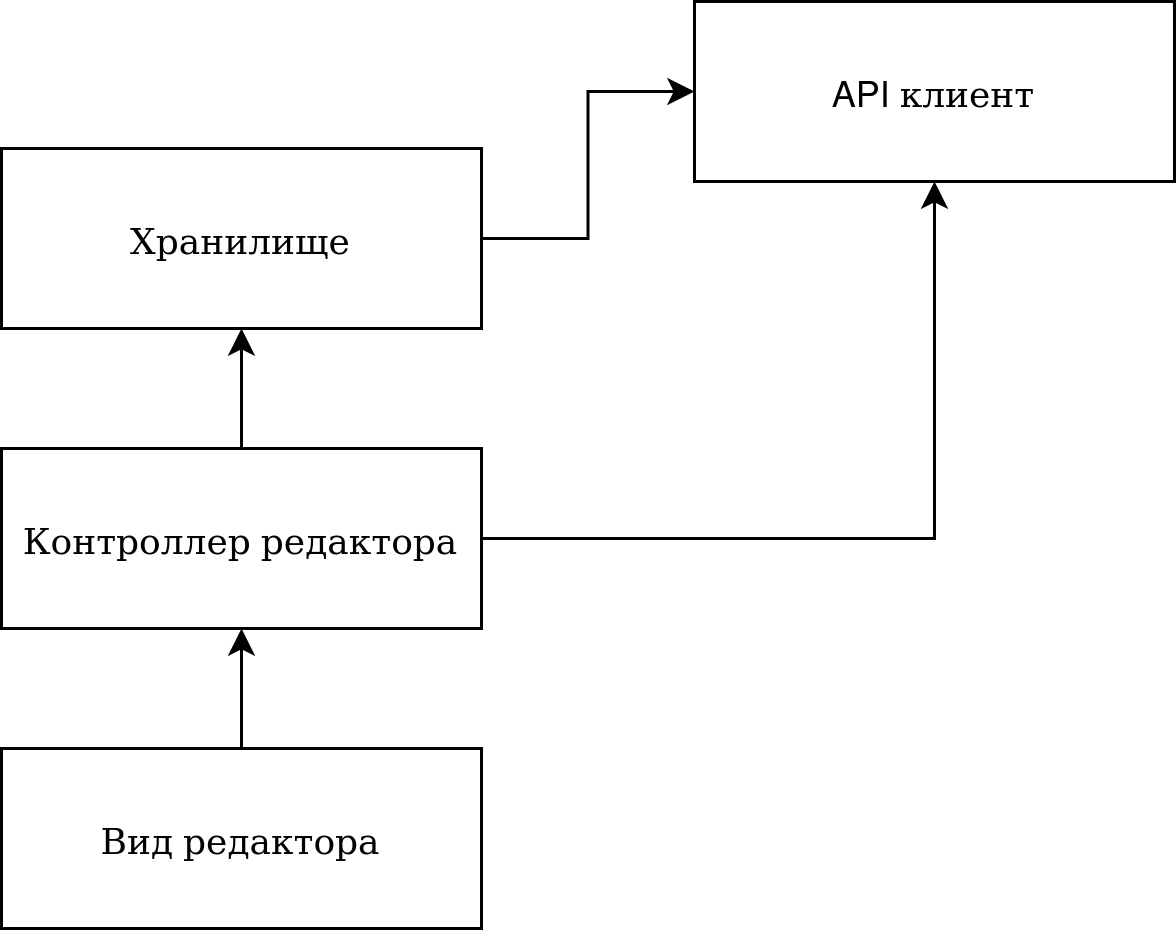
\includegraphics[width=0.8\textwidth]{structures/server/mod}
	\caption{Модульная структура серверной части конструктора}
	\label{f:mod-server-struct}
\end{figure}

Сервис ботов зависит от сервиса пользователей, который предоставляет
первому методы для авторизации пользователя. Также сервис ботов зависит
от модуля компонентов, который описывает структуры компонентов и
реализует их логику выполнения.

Для выполнения логики ботов сервис, обслуживающий ботов, вызывает
методы из модуля компонентов.

\subsubsection{Структура модуля компонентов}

Модуль компонентов состоит из следующих подмодулей:
\begin{itemize}
	\item подмодуль компонентов;
	\item подмодуль контекста;
	\item подмодуль исполнителя;
	\item подмодуль ввода-вывода.
\end{itemize}

Структура модуля компонентов представлена на рисунке~\ref{f:mod-comp-struct}.

\begin{figure}[ht]
	\centering
	\vspace{\toppaddingoffigure}
	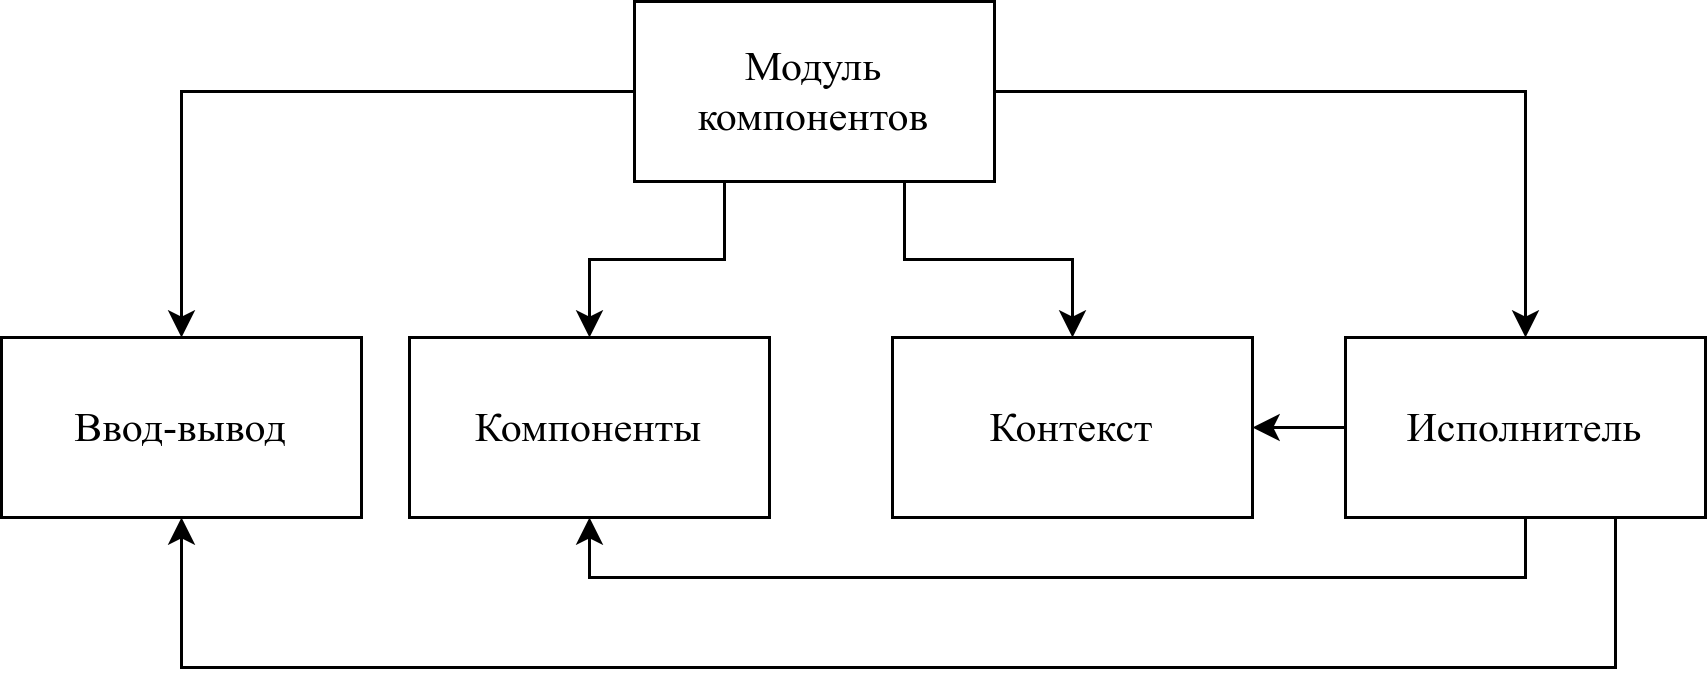
\includegraphics[width=0.8\textwidth]{structures/server/mod-comp}
	\caption{Структура модуля компонентов}
	\label{f:mod-comp-struct}
\end{figure}

Подмодуль компонентов содержит структуру и реализацию логики
компонентов. Каждый компонент реализует общий интерфейс компонента,
который определен в данном подмодуле.

В данном подмодуле определены следующие компоненты:
\begin{itemize}
	\item 	компонент ввода текста;
	\item 	компонент отправки сообщения;
	\item 	компонент вывода кнопок;
	\item 	компонент форматирования;
	\item 	компонент точки входа;
	\item 	компонент условия.
\end{itemize}

Подмодуль ввода-вывода предоставляет интерфейс, через который
окружение обменивается данными с рядом компонентов.

Подмодуль контекста содержит методы для работы с контекстом.
Контекст в рамках бота – память, с которой работают компоненты:
компоненты получают из контекста данные для выполнения и записывают в
него результат.

Исполнитель представляет собой объект, который содержит в себе
контекст и интерфейс ввода-вывода. Через него происходит выполнение
компонентов.


\subsubsection{Алгоритмы функционирования серверной части конструктора}

Пользователь конструктора взаимодействует с сервисом ботом, который
контролирует изменение данных и состояние ботов.
Схема алгоритма обработки запросов от пользователей сервиса ботов
представлен на рисунке~\ref{f:bot-service-alg}.

\begin{figure}[hp]
	\centering
	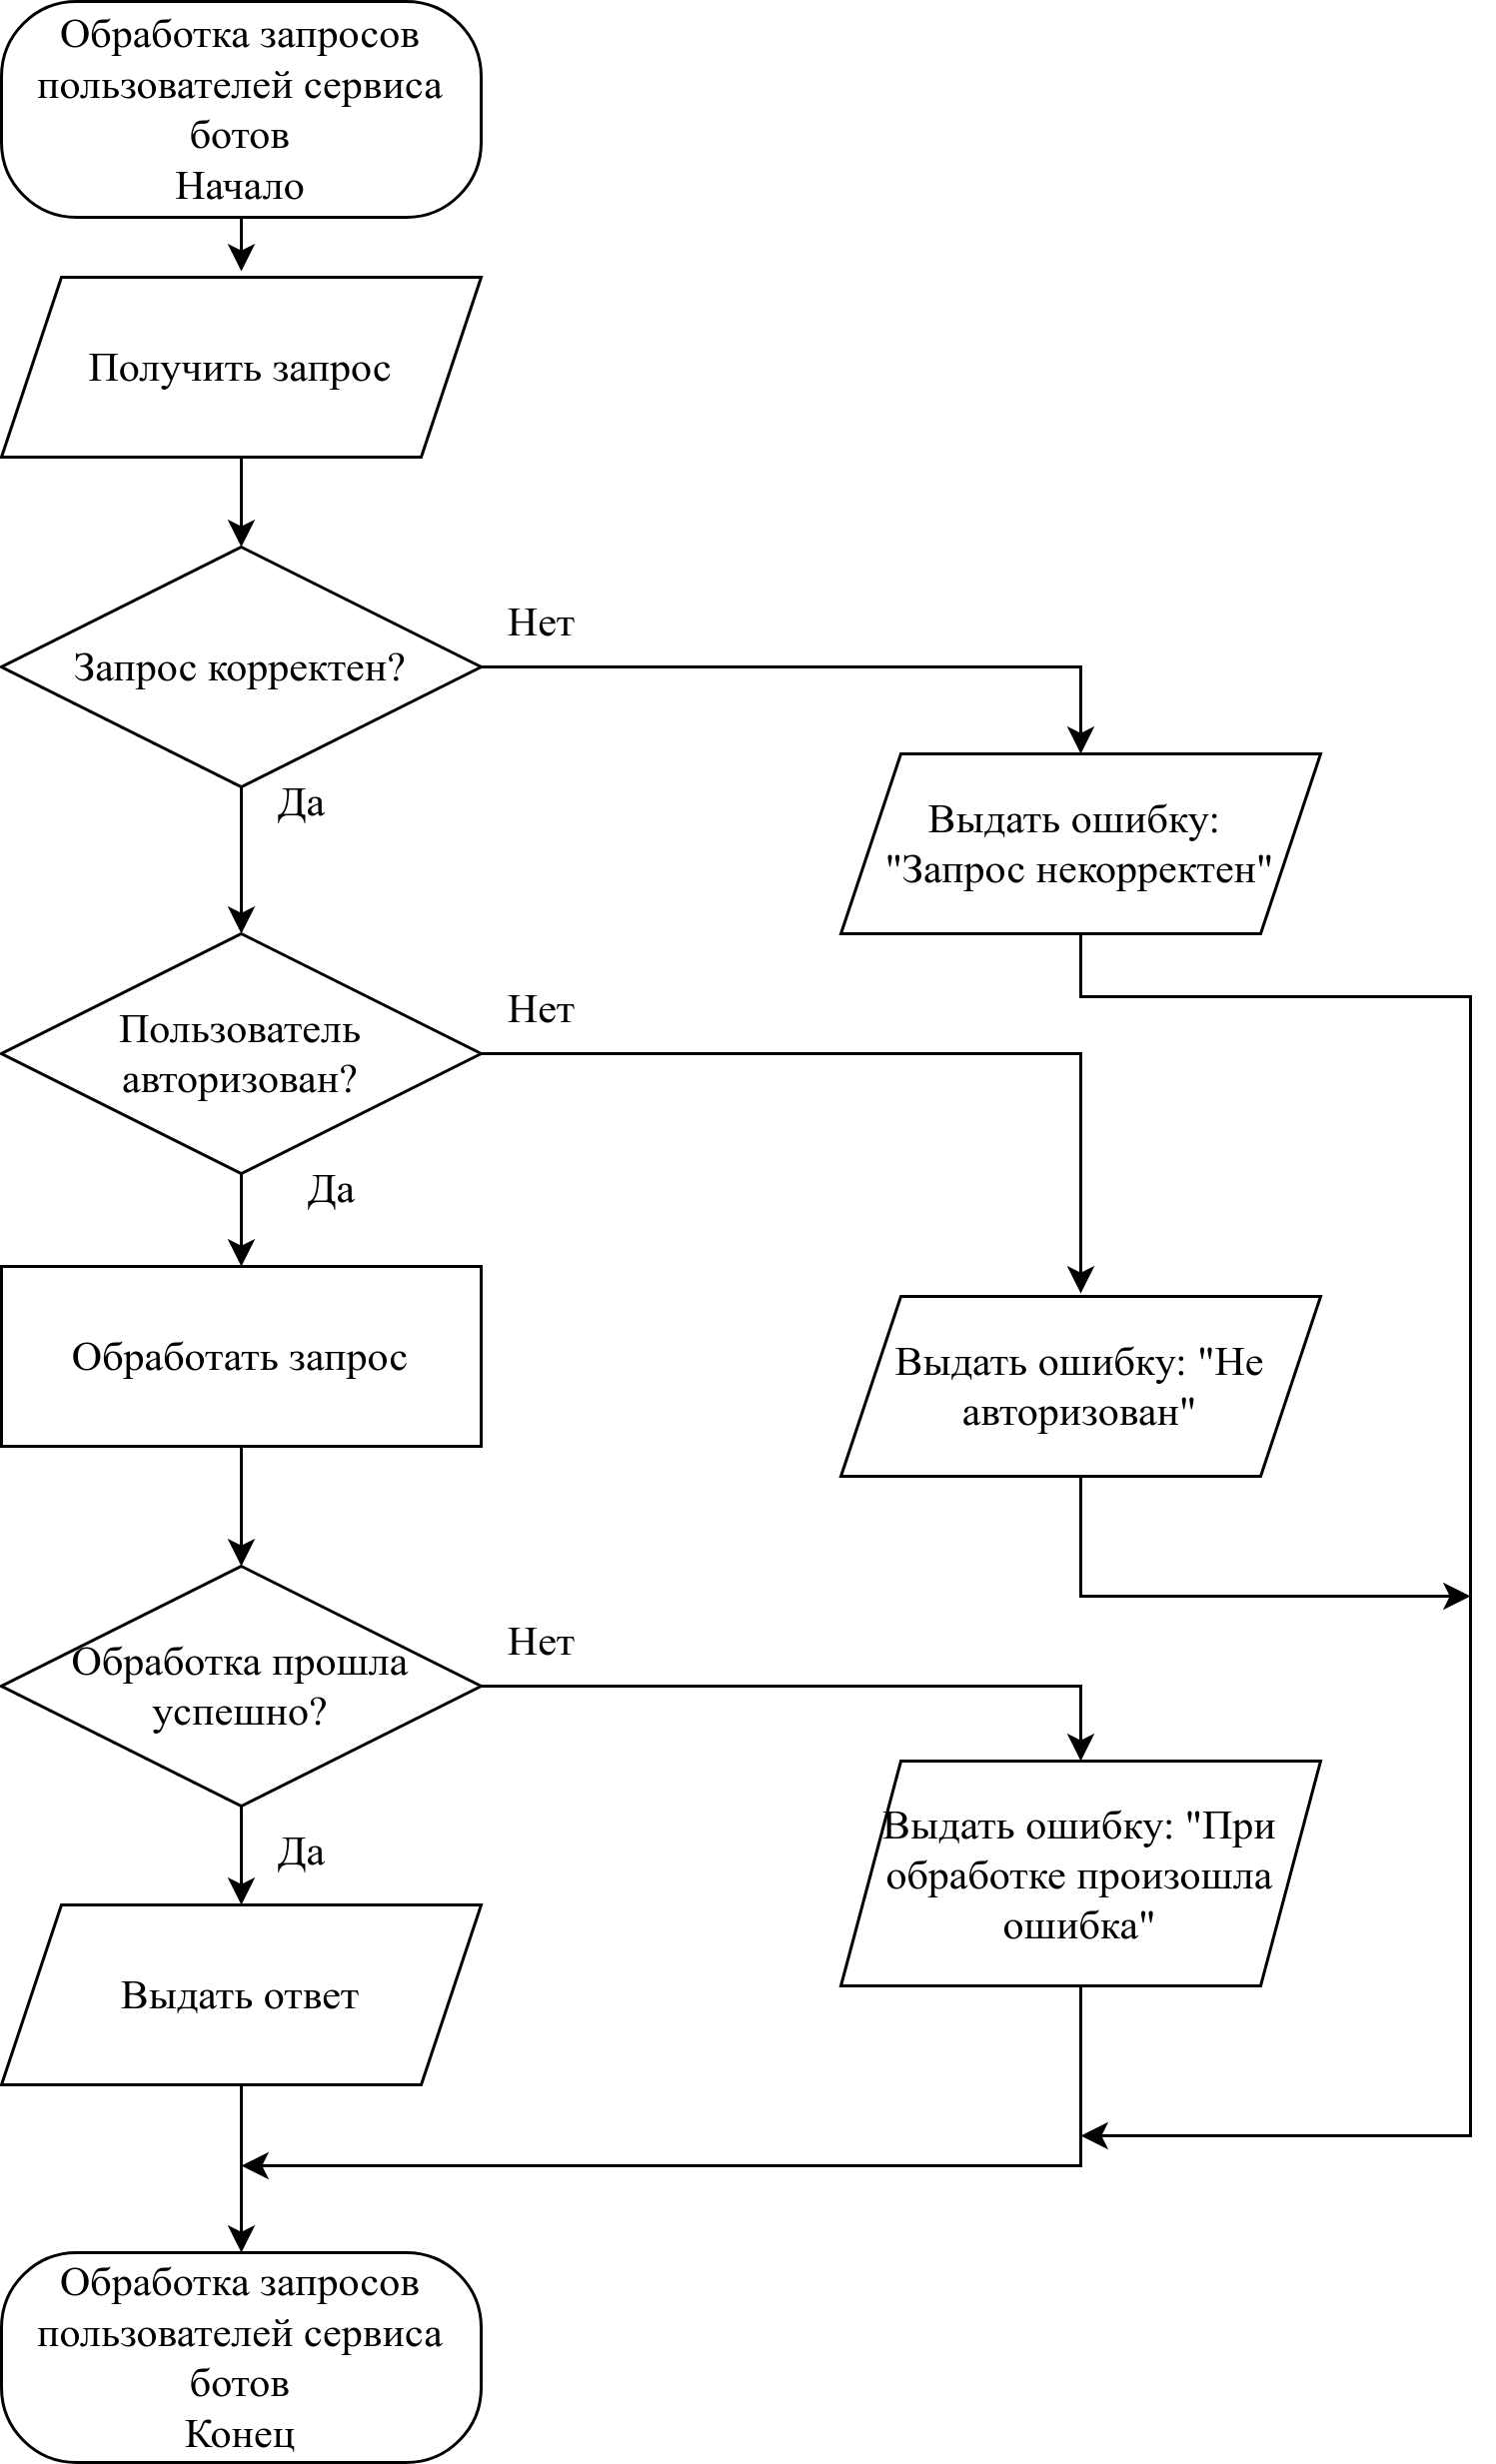
\includegraphics[height=0.9\textheight]{bot-service-alg}
	\caption{Схема алгоритма обработки запросов от пользователей сервиса ботов}
	\label{f:bot-service-alg}
\end{figure}

При получении запроса проверяется его корректность.
Если запрос не корректен, например, такое обращение не доступно, то
выводится соответствующая ошибка. Чтобы обработка прошла успешно, пользователь
должен быть авторизован в системе. В случае успешной обработки запроса выдается
ответ, иначе - ошибка.


При взаимодействии Telegram пользователя с ботом происходит
отправка запросов сервису, обслуживающему ботов, который в дальнейшем
обрабатывает данное событие. Схема алгоритма обработки запросов от
пользователя бота представлен на рисунке~\ref{f:bot-worker-alg}.


\begin{figure}[hp]
	\centering
	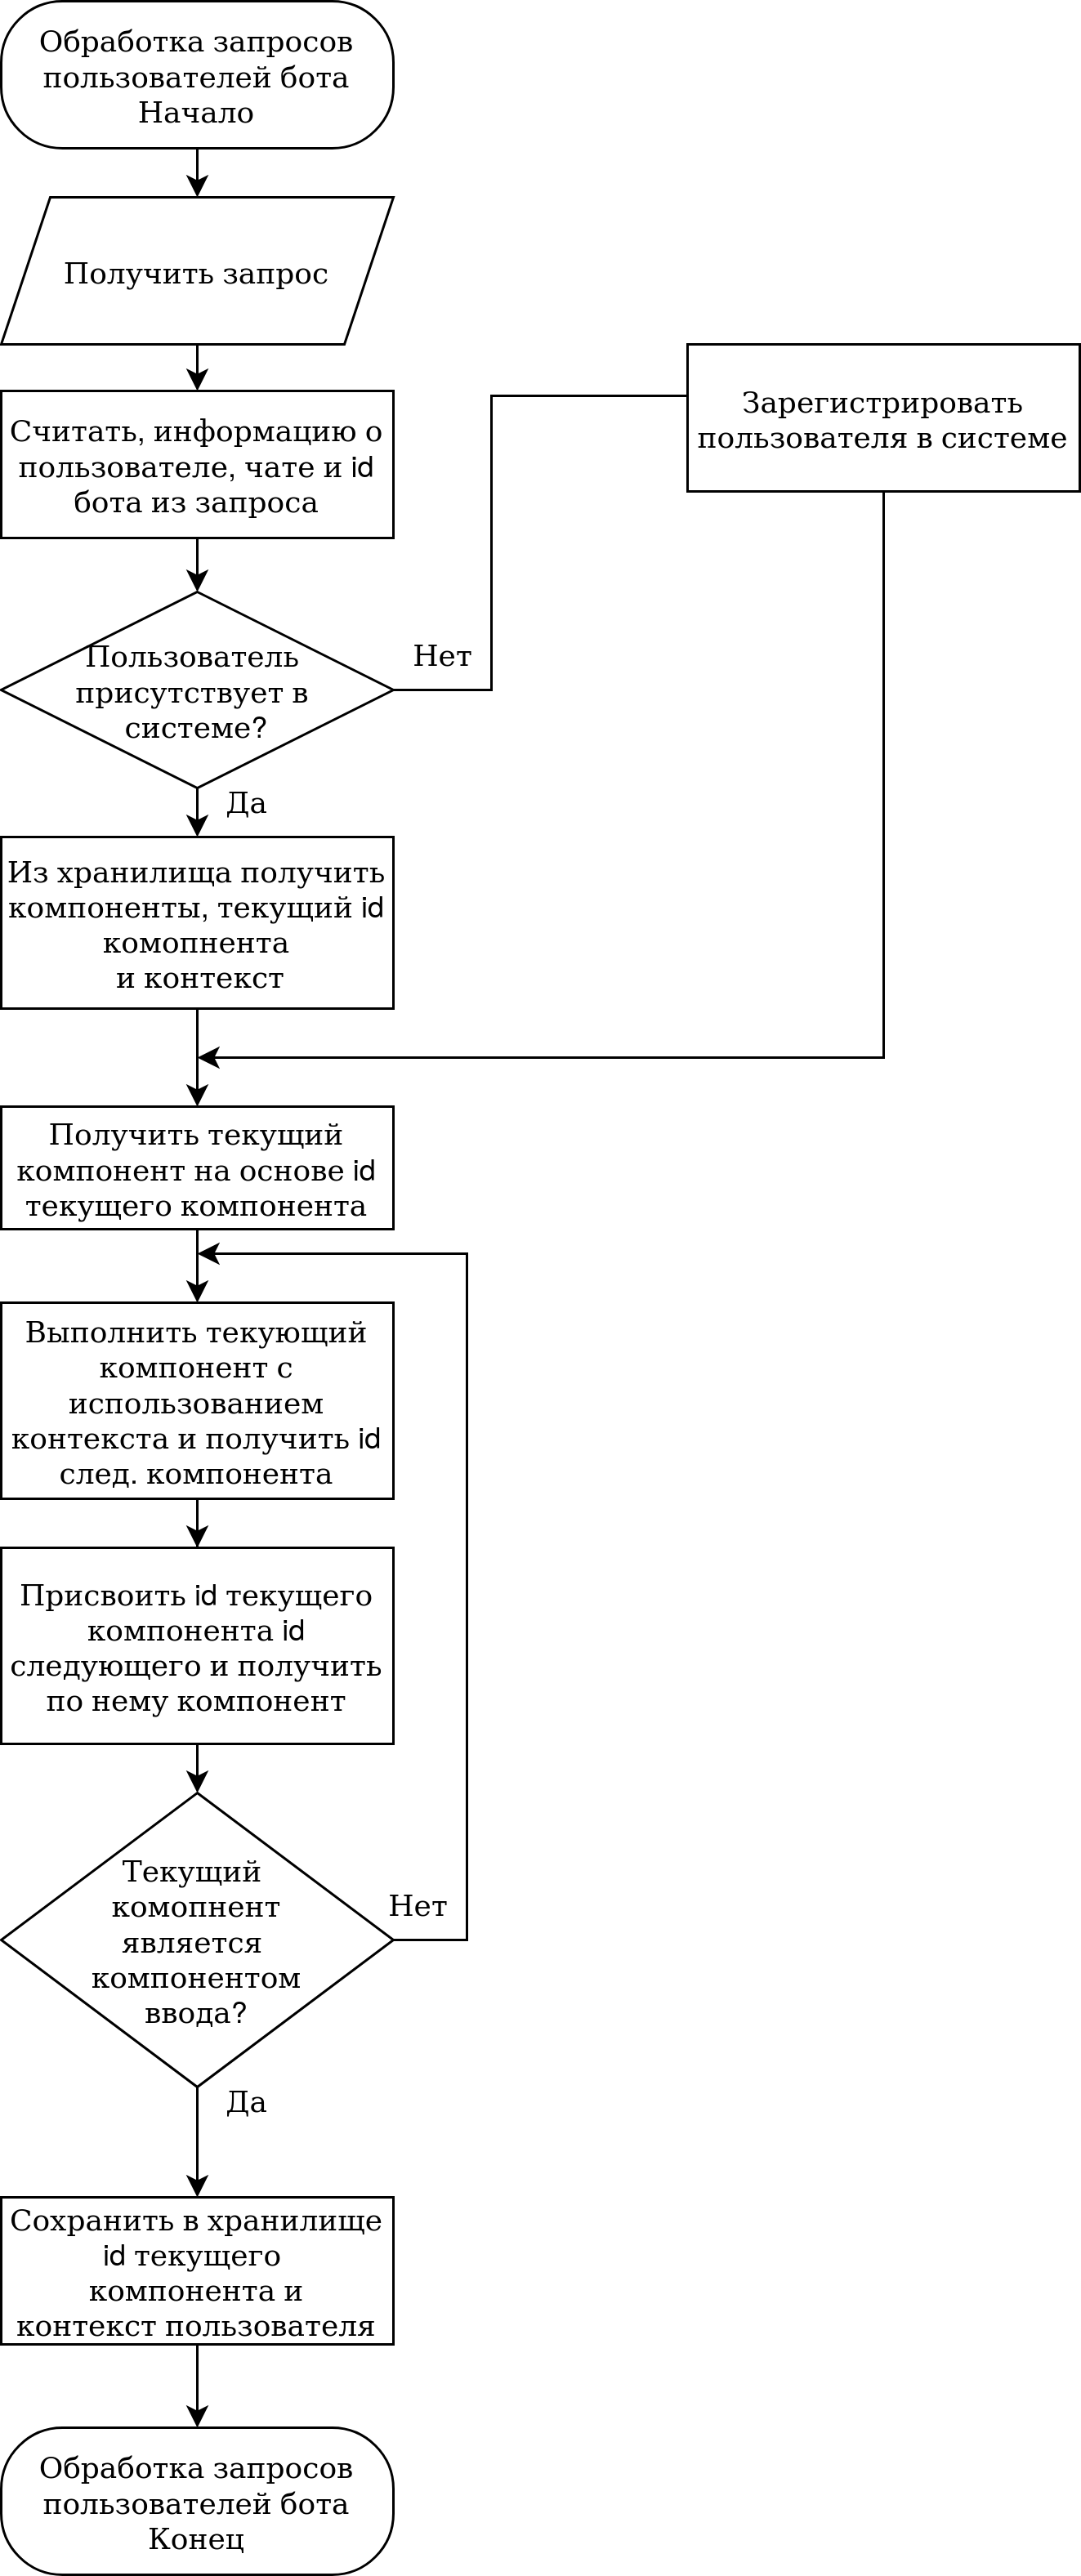
\includegraphics[height=0.9\textheight]{bot-worker-alg}
	\caption{Схема алгоритма обработки запросов от пользователей ботов}
	\label{f:bot-worker-alg}
\end{figure}

При принятии события сервисом происходит считывание следующих
данных:
\begin{itemize}
	\item информация о пользователе;
	\item информация о чате;
	\item id бота, от которого пришло сообщение.
\end{itemize}

На основе этих данных из хранилища идёт получение следующих
данных:
\begin{itemize}
	\item контекст пользователя;
	\item id текущего компонента пользователя;
	\item компонентов бота.
\end{itemize}

На основании id текущего компонента происходит получение текущего
компонента, который затем выполняется. Результат выполнения представляет
собой id следующего компонента, который присваивается текущему.

На основании следующего компонента принимается решение: если
компонент ожидает ввода каких-либо данных, то алгоритм заканчивается с
сохранением контекста и id текущего компонента, иначе идет выполнение
следующего компонента.

\newpage


\subsubsection{Обеспечение защиты информации клиентов конструктора}

Для обеспечения защищенного хранения паролей в базе данных используется
адаптивная криптографическая хеш-функция bcrypt \refref{ref:bcrypt}.

Функция основана на шифре Blowfish.
Для защиты от атак с помощью радужных таблиц bcrypt использует соль (salt);
кроме того, функция является адаптивной,
время её работы легко настраивается и её можно замедлить,
чтобы усложнить атаку перебором \refref{ref:bcrypt}.

Функция принимает три параметра: стоимость(cost), соль и пароль.
Алгоритм хеширования состоит из следующих шагов \refref{ref:bcrypt}:
\begin{enumerate}
	\item
	      инициализация состояния Blowfish с помощью дорогостоящего алгоритма настройки ключей;
	      результат состоит из массива P, состоящего из 18 подключей, и четырех S-боксов;
	\item шифрование текста «OrpheanBeholderScryDoubt» 64 раза с помощью стандартного
	      Blowfish в режиме простой замены;
	\item результат состоит из конкатенации стоимости, соли и зашифрованного текста
	      «OrpheanBeholderScryDoubt».

\end{enumerate}

Дорогостоящий алгоритм настройки ключей включает в себя следующие шаги
\refref{ref:bcrypt}:
\begin{enumerate}
	\item инициализация подключей P и S-боксов шестнадцатеричными цифрами числа $\pi$;
	\item перестановка P и S на основе пароля и соли: ExpandKey(P, S, password, salt);
	\item повторение $2^{cost}$ раз следующих шагов:
	      \begin{enumerate}
		      \item перестановка P и S на основе пароля: ExpandKey(P, S, password, 0);
		      \item перестановка P и S на основе соли: ExpandKey(P, S, salt, 0).
	      \end{enumerate}
\end{enumerate}

Алгоритм ExpendKey
\refref{ref:bcrypt}:
\begin{enumerate}
	\item смешивание пароля с массивом подключей P;
	\item
	      разбиение соли на две равные части;
	\item инициализация буфера для хранения блоков;
	\item циклическое смешивание внутреннего состояния с P, используя половины соли;
	\item циклическое смешивание зашифрованного состояния с внутренними S-блоками состояния,
	      используя половины соли.
\end{enumerate}

Аутентификация пользователя происходит по паролю и логину.
Отправленный пароль после хеширования
сравнивается с хешем из базы данных, и в случае успеха генерируется токен доступа.
Этот токен временно сохраняется в базе данных, а его копия выдается пользователю.
Используя токен, пользователь может получать доступ к функциям сервиса ботов.




\subsection{Программная реализация клиентской части конструктора}

В данном подразделе обосновывается выбор инструментов
разработки клиентской части конструктора, а также демонстрируется
итоговый дизайн пользовательского интерфейса.


\subsubsection{Выбор инструментов разработки}

В браузере доступны следующие инструменты для создания веб-приложения:
\begin{itemize}
	\item HTML;
	\item CSS;
	\item JavaScript.
\end{itemize}

HTML (HyperText Markup Language — «язык гипертекстовой разметки»)
— самый базовый строительный блок Веба. Он определяет содержание и
структуру веб-контента.

Cascading Style Sheets (CSS) — это язык иерархических правил,
используемый для представления внешнего вида документа, написанного на
HTML. CSS описывает, каким образом элемент должен отображаться на
экране, на бумаге, голосом или с использованием других медиа средств.

JavaScript — это легковесный, интерпретируемый или JIT-
компилируемый, объектно-ориентированный язык с функциями первого
класса. Наиболее широкое применение находит как язык сценариев веб-
страниц. JavaScript это прототипно-ориентированный, мультипарадигменный
язык с динамической типизацией, который поддерживает объектно-
ориентированный, императивный и декларативный (например,
функциональное программирование) стили программирования.

Основной недостаток JavaScript – это динамическая типизация, при
которой переменная связывается с типом в момент присваивания значения, а
не в момент объявления переменной. Это особенность JS приводит к
достаточно долгой отладке кода при возникновении ошибки.

Для решения этой проблемы был выбран язык TypeScript –
компилируемый язык с возможностью явного статического назначения типов.
Статическая типизация устраняет основной недостаток JS, а компиляция
позволяет выявить некоторые ошибки до запуска приложения. Также он
совместим с JS.

Среди инструментов, облегчающих разработку клиентских приложений
в браузере, имеются:

\begin{itemize}
	\item Vue - JavaScript-фреймворк с открытым исходным кодом для
	      создания пользовательских интерфейсов. Легко интегрируется в проекты с
	      использованием других JavaScript-библиотек. Может функционировать как
	      веб-фреймворк для разработки одностраничных приложений в реактивном
	      стиле.
	\item Angular - открытая и свободная платформа для разработки веб-
	      приложений, написанная на языке TypeScript, разрабатываемая командой из
	      компании Google, а также сообществом разработчиков из различных
	      компаний.
	\item React - JavaScript-библиотека с открытым исходным кодом для
	      разработки пользовательских интерфейсов. React разрабатывается и
	      поддерживается Facebook, Instagram и сообществом отдельных разработчиков
	      и корпораций. React может использоваться для разработки одностраничных и
	      мобильных приложений. Его цель — предоставить высокую скорость
	      разработки, простоту и масштабируемость.
	\item SolidJS – это легковесная JavaScript библиотека для создания
	      пользовательских интерфейсов. SolidJS вдохновлен библиотекой React, но
	      нацелен на предоставление более простой и эффективной модели
	      программирования.
\end{itemize}

В качестве сравнения данных библиотек и фреймворков выделим
следующие критерии:
\begin{itemize}
	\item поддержка реактивности;
	\item сложность изучения;
	\item производительность;
	\item потребление памяти.
\end{itemize}

Под реактивностью понимается обновления отображения при
изменении привязанных данных.

Angular является фреймворком для создания крупных браузерных
решений. Он имеет довольно много возможностей и из-за этого имеет
довольно большой размер и сложен для обучения.

Vue является фреймворком для создания реактивных приложений.
Имеет много оптимизаций в своей основе: кэширование вычисляемых
свойств, умная перерисовка – перерисовываются только нужные узлы, что
позволяет работать приложению довольно быстро. Также легок в обучении и
не требует много памяти.

React является библиотекой для создания реактивных приложения.
Имеет немного низкую производительность, чем Vue, но обладает высокой
скоростью обучения и также предрасположен к низкому потреблению памяти.

SolidJS также является библиотекой для создания реактивных
приложений. Реактивность реализуется без использования виртуального
DOM, что увеличивает производительность библиотеки и уменьшает
потребление памяти.

Сравнение фреймворков и библиотек по критериям представлено в
таблице~\ref{t:comp-client-lib}.


\begin{table}[ht]
	\Large
	\begin{threeparttable}
		\caption{Сравнение фреймворков и библиотек JavaScript}
		\label{t:comp-client-lib}
		\centering
		\begin{tabularx}{\textwidth}
			{|>{}X
			|>{\centering\arraybackslash}X
			|>{\centering\arraybackslash}X
			|>{\centering\arraybackslash}X
			|>{\centering\arraybackslash}X|}
			\hline
			        &
			Vue.js  &
			React   &
			Angular &
			SolidJS                                         \\
			\hline
			Поддержка
			реактивности
			        & есть    & есть    & есть    & есть    \\
			\hline
			Сложность изучения
			        & низкая  & низкая  & высокая & низкая  \\
			\hline
			Про\-из\-во\-ди\-тель\-ность
			        & средняя & средняя & средняя & высокая \\
			\hline
			Потребление памяти
			        & низкое  & низкое  & высокое & низкое  \\
			\hline
		\end{tabularx}
	\end{threeparttable}
	\vspace{\bottompaddingoftable}
\end{table}



Исходя из таблицы можно сделать вывод, что SolidJS является самым
оптимальным выбором для разработки клиентской части для конструктора
Telegram-ботов.


\subsubsection{Дизайн пользовательского интерфейса}

На основании составленных шаблонов для интерфейса клиентской части была выполнена
их реализация и стилизация.

Для обозначения элементов интерфейса конструктора Telegram-ботов были выбраны следующие цвета:
\begin{itemize}
	\item серый;
	\item синий;
	\item зелёный;
	\item красный;
	\item желтый.
\end{itemize}

Также у каждых цветов были выбраны более светлые оттенки для обозначения фонов неактивных элементов, таких как кнопки.

Преобладающий цвет – синий, он является основным для конструктора.
Он, а также его более светлые оттенки используются
для обозначения компонентов в редакторе бота,
а также для стилизации шапки веб-приложения.
Также данный цвет служит для обозначения кнопок, которые
обеспечиваю переход на другие страницы.

Серый цвет является основным фоновым для веб-приложения,
на нём располагаются белые плитки. Плитка представляет
собой группу элементов интерфейса конструктора.

Зелёный цвет применяется для обозначения кнопок,
благодаря которым будет происходить добавление объектов
конструктора или изменение их состояния на активное.

Красный цвет служит для метки тех элементов,
которые способны удалить объекты конструктора,
или для обозначения выходов ошибок у компонентов.

Жёлтый цвет применяется для обозначения элементов интерфейса,
которые позволяют вернуться назад по страницам,
либо служат для изменения состояния
объектов конструктора на неактивное или для их индикации.

Экранные формы пользовательского интерфейса конструктора представлена
на рисунках~\ref{f:signin-page}-\ref{f:editor-page}.

{

\newcommand{\scale}{1}

\begin{figure}[p!]
	\centering
	\vspace{\toppaddingoffigure}
	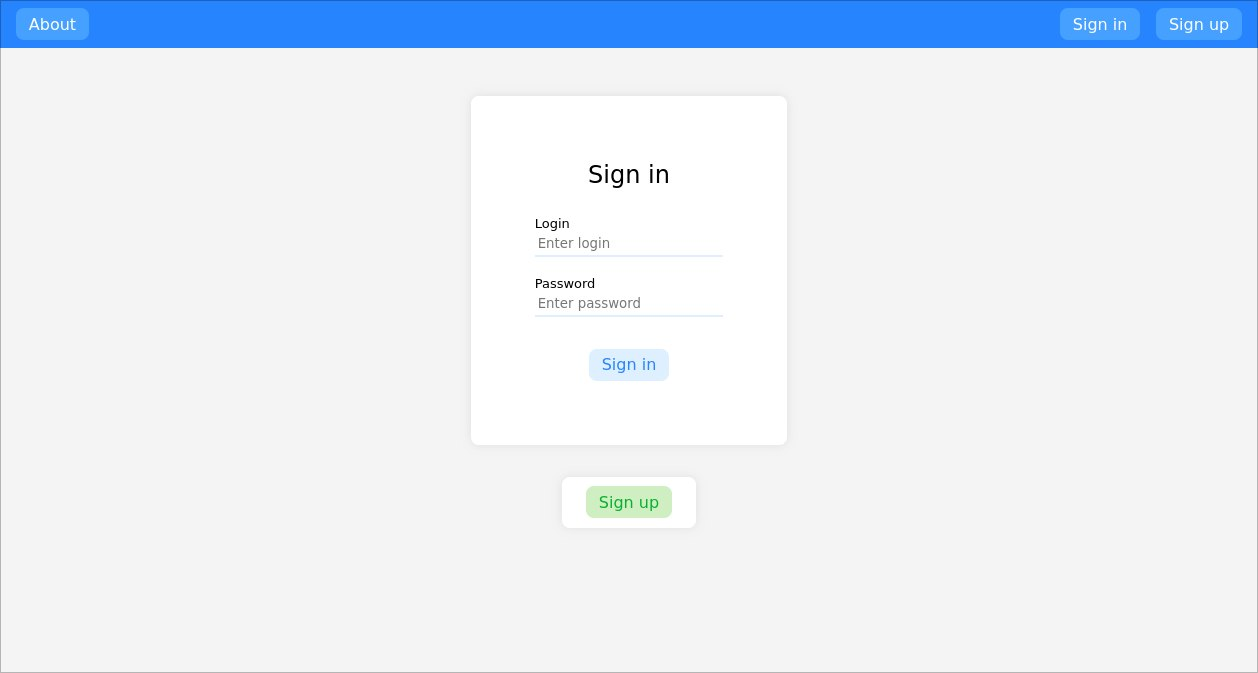
\includegraphics[width=\scale\textwidth]{/pages/signin}
	\caption{Страница входа в приложение}
	\label{f:signin-page}
\end{figure}


\begin{figure}[p!]
	\centering
	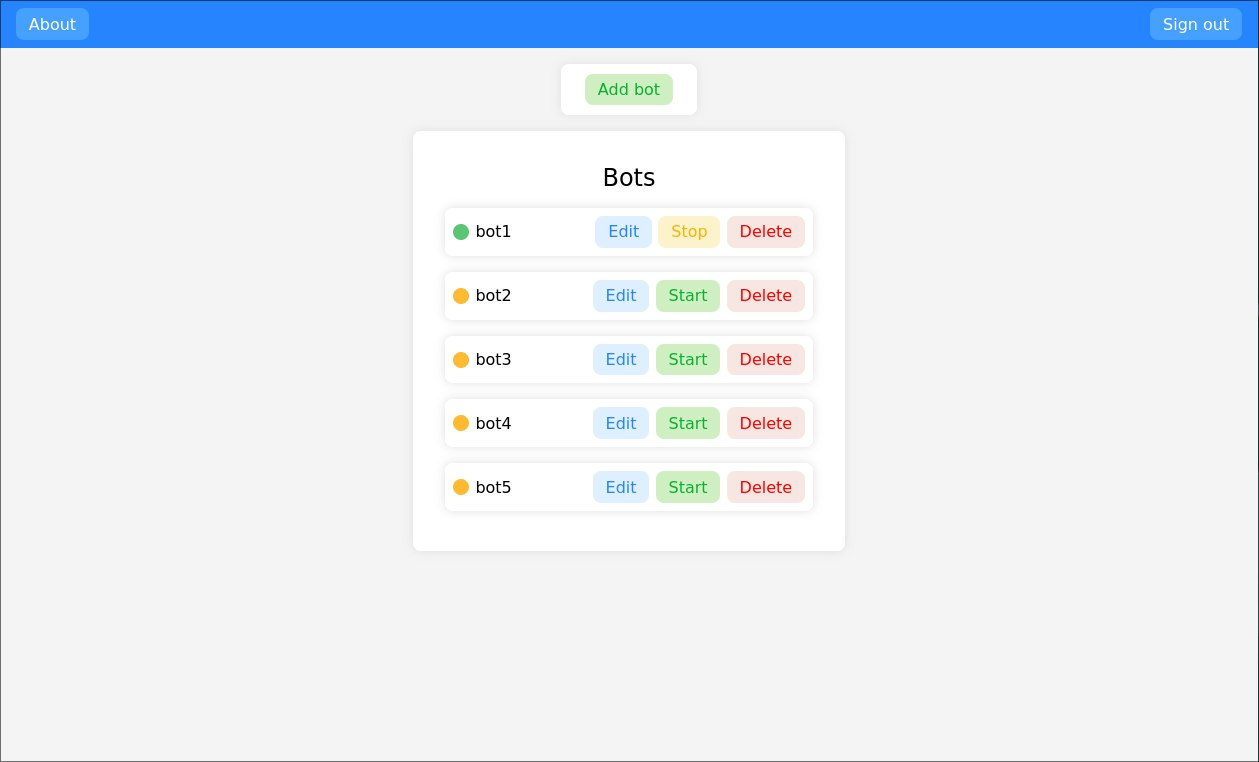
\includegraphics[width=\scale\textwidth]{/pages/bot-list}
	\caption{Страница списка ботов}
	\label{f:bot-list-page}
\end{figure}

\begin{figure}[p!]
	\centering
	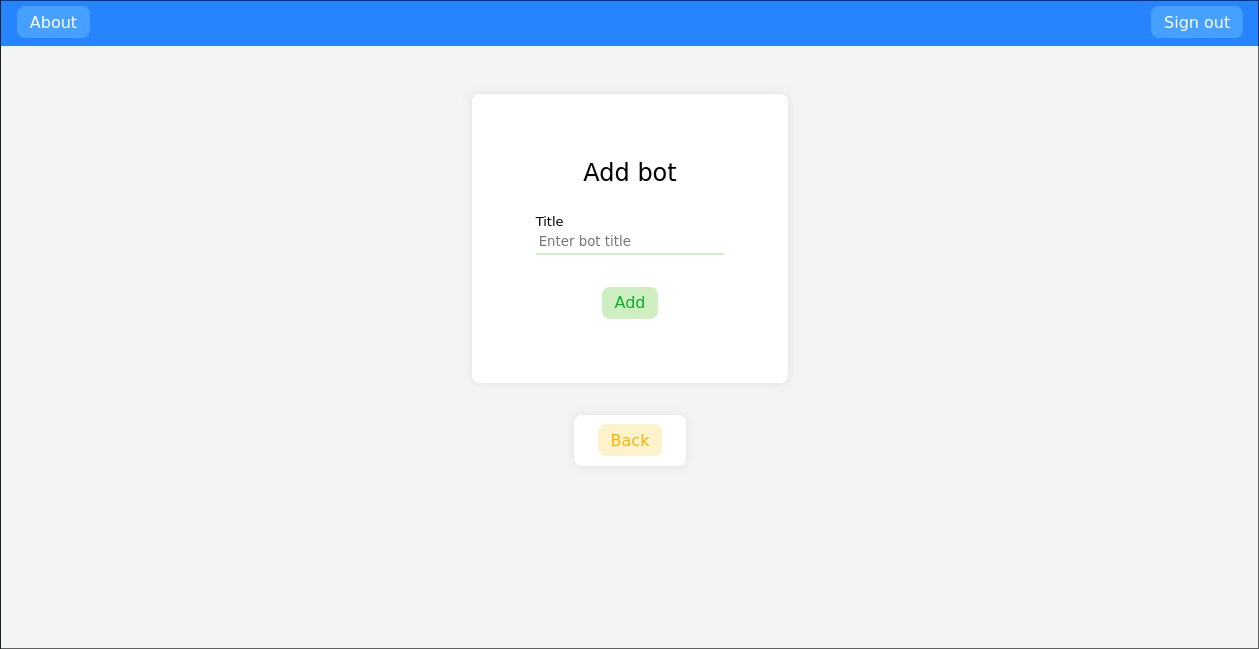
\includegraphics[width=\scale\textwidth]{/pages/add-bot}
	\caption{Страница добавления бота}
	\label{f:add-bot-page}
\end{figure}

\begin{figure}[p!]
	\centering
	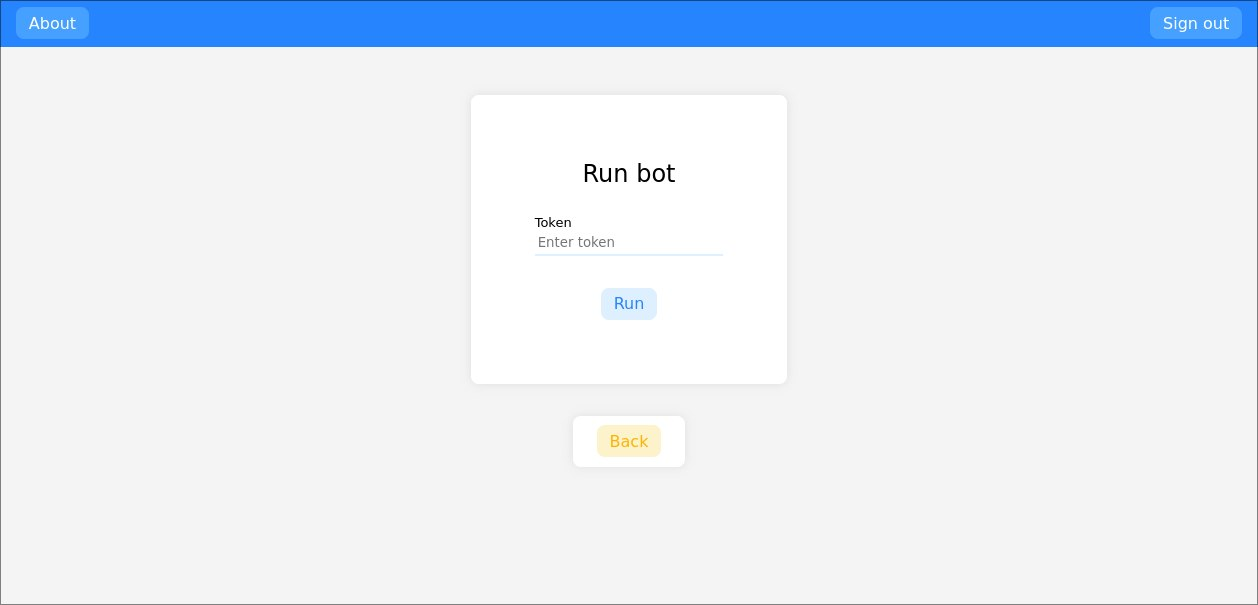
\includegraphics[width=\scale\textwidth]{/pages/run-bot}
	\caption{Страница запуска бота}
	\label{f:run-bot-page}
\end{figure}


\begin{figure}[ht]
	\centering
	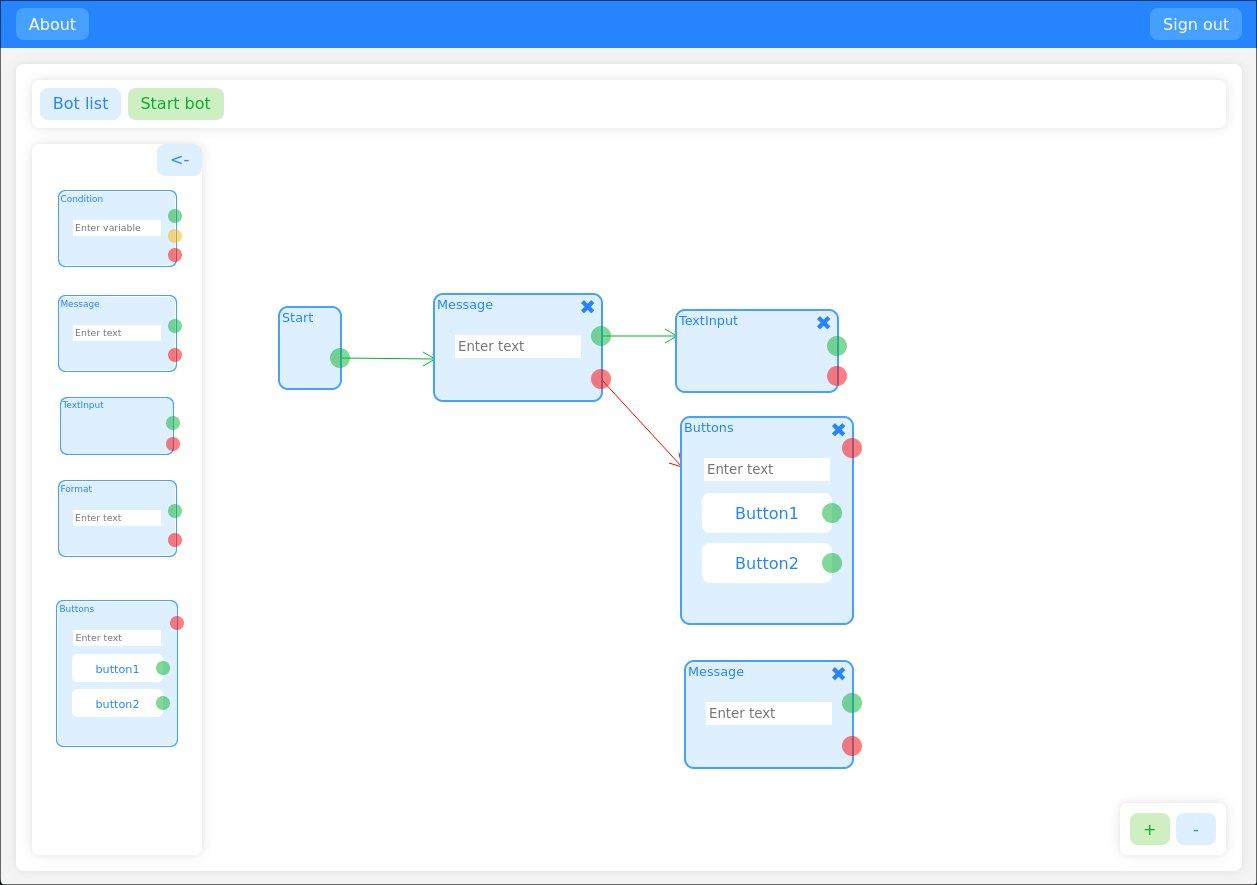
\includegraphics[width=\scale\textwidth]{/pages/editor}
	\caption{Страница визуального редактора}
	\label{f:editor-page}
\end{figure}

}



\newpage

\section*{Выводы}

В данном разделе были рассмотрены основные
инструменты и средства, используемые при создании
конструктора. Были рассмотрены аналоги, их плюсы и
минусы.

Был выбран формат передаваемых данных между серверной и клиентской
частями конструктора. У серверной части были выделены и разработаны
программные интерфейсы,
благодаря которым клиентская часть может обмениваться данными с сервисами.

На основе разработанных структур приложения, алгоритмов
функционирования и диаграмм состояний была выполнена программная реализация конструктора.
Листинг кода представлен в приложении .

